\documentclass[a4paper]{report}
\usepackage[group-separator={,},group-minimum-digits={3}]{siunitx}
\usepackage[utf8]{inputenc}
\usepackage[dvipsnames, table]{xcolor}
\usepackage{tcolorbox}
\usepackage{multicol}
\usepackage{lipsum}
\usepackage[margin=0.2in]{geometry}
\usepackage{xstring}
\usepackage{xifthen}
\usepackage[dvipsnames]{xcolor}
\usepackage{setspace}
\usepackage{amsmath}
\usepackage{enumitem}
\pagenumbering{gobble}
\setlength{\columnsep}{1.5cm}
\setlength{\columnseprule}{0.2pt}
\usepackage{latexsym}
\usepackage{hyperref}
\usepackage[none]{hyphenat}
\usepackage{graphicx}
\usepackage{etoolbox}
\usepackage{pgffor}
\usepackage{titlepic}
\usepackage{enumitem}
\usepackage[outline]{contour}

\setlist{nosep}

\hypersetup{
    colorlinks,
    citecolor=black,
    filecolor=black,
    linkcolor=black,
    urlcolor=black
}

\usepackage[default]{sourcesanspro}

\makeatletter
\def\@makechapterhead#1{%
  %\vspace*{5\p@}%
  {\parindent \z@ \raggedleft \normalfont
    \ifnum \c@secnumdepth >\m@ne
        \large\bfseries #1
        \par\nobreak
%        \vskip 10\p@
        \rule{\columnwidth}{.1pt}%
%        \vskip 10\p@
    \fi
    \interlinepenalty\@M
%    \large \bfseries \MakeUppercase{#1}\par\nobreak
%    \vskip 5\p@
  }}
\makeatother

\usepackage{enumitem}
\setitemize{noitemsep,topsep=0pt,parsep=0pt,partopsep=0pt}
\usepackage{graphicx}


\title{Fire Emblem Three Houses Any\% Cindered Shadows Normal/Classic}
\author{Mr.Tyton}
\titlepic{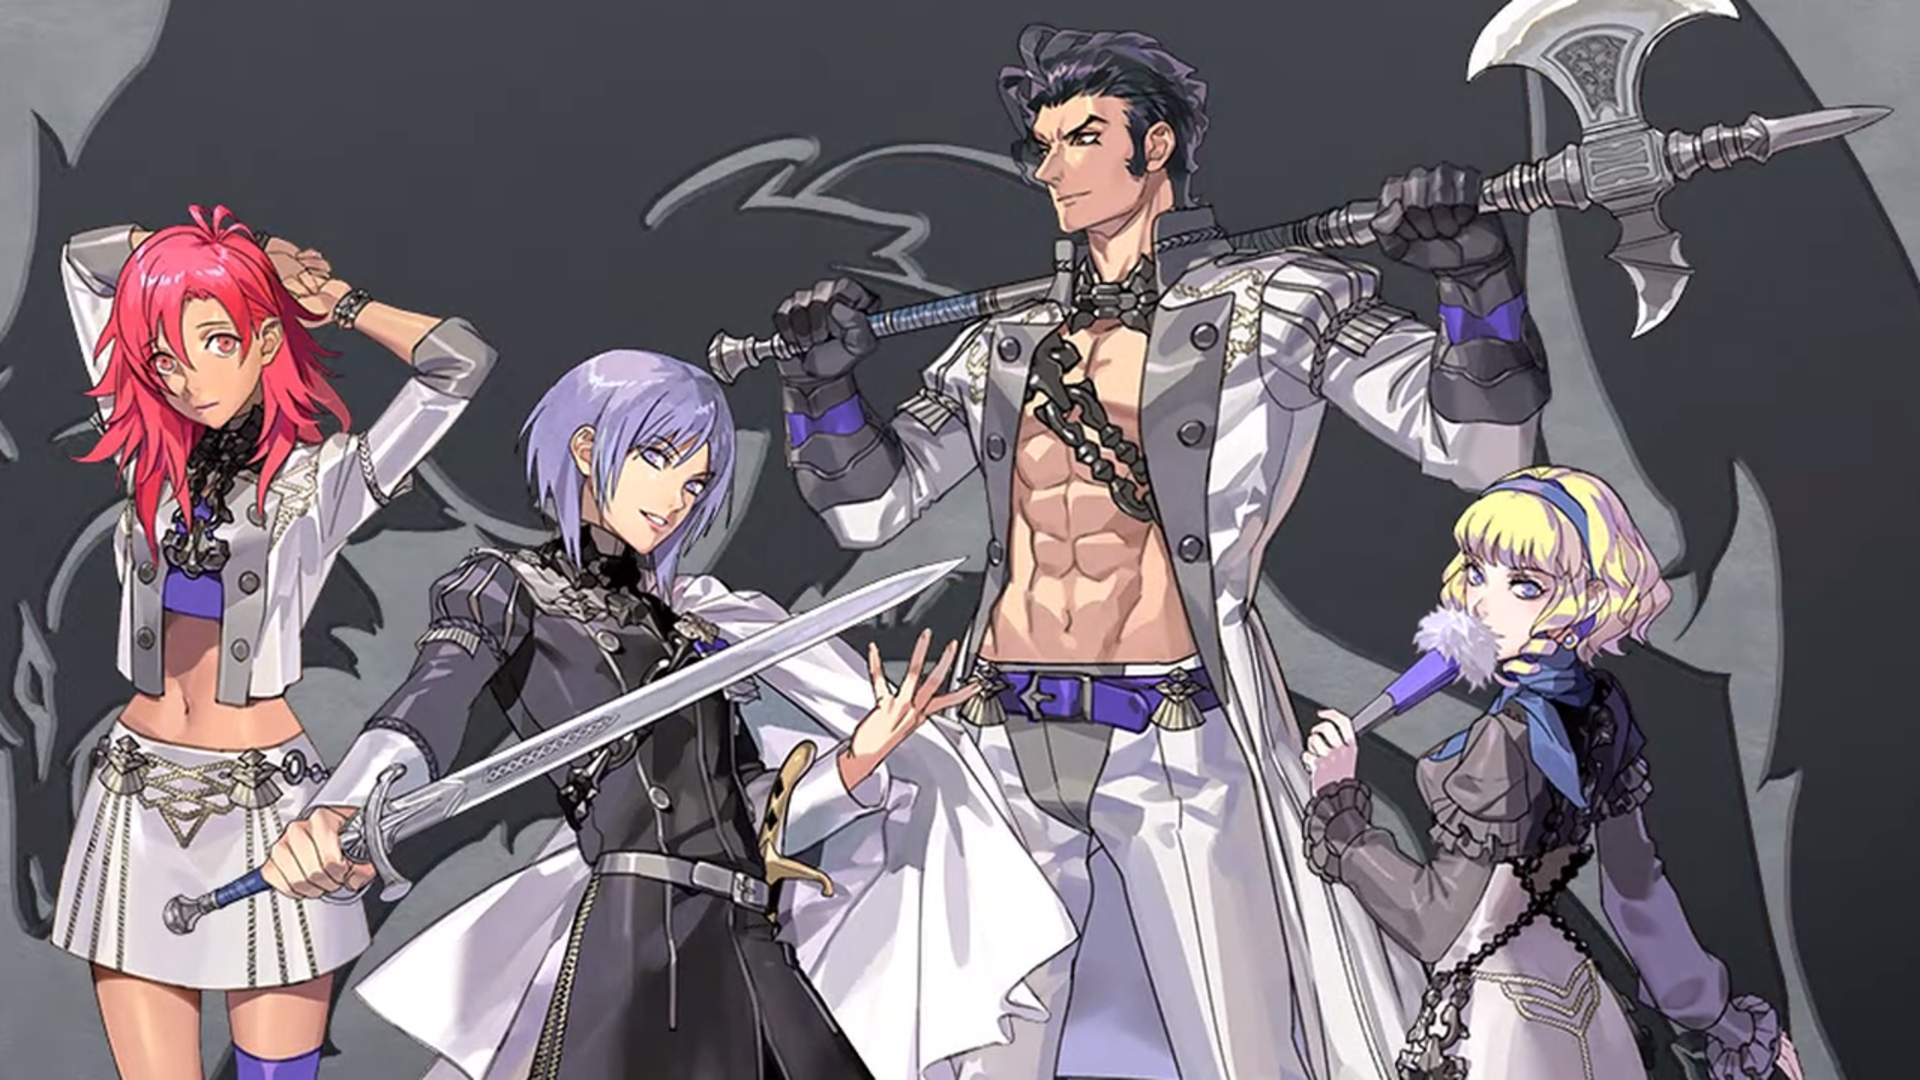
\includegraphics[width=\textwidth]{./Cindered Shadows/cindered_shadows.jpg}}
\begin{document}
\singlespacing
\maketitle
\tableofcontents
\makeatletter
\patchcmd{\chapter}{\if@openright\cleardoublepage\else\clearpage\fi}{}{}{}
\makeatother

\newcounter{chaptercount}

\newenvironment{battlespecial}[1]{\begin{tcolorbox}[title=\begin{center}#1\end{center},colbacktitle=red!50!white]}{\end{tcolorbox}}
\newenvironment{battle}[1]{\refstepcounter{chaptercount} \begin{tcolorbox}[title=\begin{center}Chapter \thechaptercount\ - #1\end{center},colbacktitle=red!50!white]}{\end{tcolorbox}}


\newcommand{\battleinfo}[3]{Goal: \ifthenelse{\equal{#1}{rout}}{Rout the Enemy}{\ifthenelse{\equal{#1}{commander}}{Defeat the Commander}{#1}} \newline Turns: #2 \newline Units: #3}

\newenvironment{shop}[1]{\begin{tcolorbox}[title=\begin{center}SHOP\, #1 GOLD\end{center},colbacktitle=OliveGreen!50!white]}{\end{tcolorbox}}

\newcommand{\cs}[1][]{\textbf{CS}%
	\ifthenelse{\isempty{#1}}{}{ (#1)}%
}

% Console Buttons
\newcommand{\down}{\textbf{$\downarrow$}}
\newcommand{\abutton}{\textbf{A}}
\newcommand{\bbutton}{\textbf{B}}

% Instruct
\newcommand{\autoInstruct}{\textbf{Auto-Instruct}}

% -----------------------

\newcommand{\createCharacter}[2]{%
\expandafter\newcommand\csname #1\endcsname{\textbf{\textcolor[RGB]{#2}{#1}}} %
\expandafter\newcommand\csname #1f\endcsname{\item \textbf{\textcolor[RGB]{#2}{#1}}:}
}


% Byleth
\createCharacter{Byleth}{73,114,132}

% Black Eagle
\createCharacter{Edelgard}{254,255,244}
\createCharacter{Hubert}{45,60,62}
\createCharacter{Ferdinand}{254,180,116}
\createCharacter{Linhardt}{71,99,82}
\createCharacter{Caspar}{168,228,226}
\createCharacter{Bernadetta}{158,127,167}
\createCharacter{Dorothea}{119,85,87}
\createCharacter{Petra}{129,68,98}

% Blue Lions
\createCharacter{Dimitri}{209, 199, 36}
\createCharacter{Dedue}{231,232,224}
\createCharacter{Felix}{63,64,96}
\createCharacter{Ashe}{181,189,198}
\createCharacter{Sylvain}{229,111,85}
\createCharacter{Mercedes}{244,220,196}
\createCharacter{Annette}{246,166,125}
\createCharacter{Ingrid}{248,230,158}

% Black Deer
\createCharacter{Claude}{76,67,66}
\createCharacter{Lorenz}{115,115,172}
\createCharacter{Raphael}{239,216,162}
\createCharacter{Ignatz}{198,198,157}
\createCharacter{Lysithea}{254,252,253}
\createCharacter{Marianne}{170,208,250}
\createCharacter{Hilda}{252,175,183}
\createCharacter{Leonie}{241,125,91}

% The Church of Seiros
\createCharacter{Seteth}{111,178,157}
\createCharacter{Flayn}{158,239,205}
\createCharacter{Hanneman}{151,151,151}
\createCharacter{Manuela}{175,154,127}
\createCharacter{Gilbert}{247,170,135}
\createCharacter{Alois}{134,123,104}
\createCharacter{Catherine}{244,234,199}
\createCharacter{Shamir}{86,89,126}
\createCharacter{Cyril}{70,62,60}

% Ashen Wolves
\createCharacter{Yuri}{172,160,207}
\createCharacter{Balthus}{52,57,64}
\createCharacter{Constance}{255,253,174}
\createCharacter{Hapi}{254,89,109}

% Miscellaneous Character
\createCharacter{Anna}{216,93,119}

% -----------------------

% ROUTE SPECIFIC COMMANDS

% Define the dancer for this route
\newcommand{\dancer}{\Sylvianf}


% -----------------------


\newcommand{\enemy}[1]{\textbf{\textcolor{red}{#1}}}
\newcommand{\autoturnCharge}{\turn{\autoCharge}}
\newcommand{\autoCharge}{\item Auto-Battle: Charge}
\newcommand{\autoUnite}{\item Auto-Battle: Unite}
\newcommand{\autoFallBack}{\item Auto-Battle: Fall Back}
\newcommand{\move}[1]{\item Move #1}
\newcommand{\attack}[2]{\item Attack \enemy{#1} #2}
\newcommand{\attacks}[2]{\ Attack \enemy{#1} #2}
\newcommand{\physic}[2]{\item Physic #1 #2}
\newcommand{\recover}[2]{\item Recover #1 #2}
\newcommand{\wait}{\item Wait}
\newcommand{\turn}[1]{\item \ \begin{itemize} #1 \end{itemize}}
\newcommand{\turnend}{\item End}
\newcommand{\trade}[3]{\item Trade with #1: #2 for #3}
\newcommand{\use}[1]{\item Use #1}
\newcommand{\equip}[1]{\item Equip #1}
\newcommand{\dismount}{\item Dismount}
\newcommand{\movedismountwait}[1]{\begin{itemize}\move{#1}\dismount\wait\end{itemize}}
\newcommand{\movedismountuse}[2]{\begin{itemize}\move{#1}\dismount\use{#2}\end{itemize}}
\newcommand{\movewait}[1]{\begin{itemize}\move{#1}\wait\end{itemize}}
\newcommand{\moveuse}[2]{\begin{itemize}\move{#1}\use{#2}\end{itemize}}
\newcommand{\moveequip}[2]{\begin{itemize}\move{#1}\equip{#2}\wait\end{itemize}}
\newcommand{\moveattack}[3]{\begin{itemize}\move{#1}\attack{#2}{#3}\end{itemize}}
\newcommand{\onlyattack}[2]{\begin{itemize}\attack{#1}{#2}\end{itemize}}
\newcommand{\moverecover}[3]{\begin{itemize}\move{#1}\recover{#2}{#3}\end{itemize}}
\newcommand{\onlyphysic}[2]{\begin{itemize}\physic{#1}{#2}\end{itemize}}
\newcommand{\movephysic}[3]{\begin{itemize}\move{#1}\physic{#2}{#3}\end{itemize}}
\newcommand{\gambit}[3]{\item Gambit: #1 on #2 #3}
\newcommand{\movegambit}[4]{\begin{itemize}\move{#1}\gambit{#2}{#3}{#4}\end{itemize}}

\newcommand{\dance}[3]{\dancer \begin{itemize}\move{#1}\item Dance for #2 #3\end{itemize}}

\newcommand{\divinepulse}{\textbf{Divine Pulse}}

% Prep Macros
\newcommand{\units}[1]{\item Select Units: \begin{itemize} #1 \end{itemize}}
\newcommand{\remove}[1]{\item Remove #1}
\newcommand{\add}[1]{\item Add #1}

\newcommand{\prep}[1]{\newline Preparations: \begin{itemize} #1 \end{itemize}}
\newcommand{\inventory}[1]{\item Inventory: \begin{itemize} #1 \end{itemize}}
\newcommand{\battalion}[1]{\item Battalion: \begin{itemize} #1 \end{itemize}} 
\newcommand{\abilities}[1]{\item Abilities: \begin{itemize} #1 \end{itemize}}
\newcommand{\armory}[1]{\item Armory: \begin{itemize} #1 \end{itemize}}
\newcommand{\repair}[1]{\item Repair: \begin{itemize} #1 \end{itemize}}
\newcommand{\forge}[1]{\item Forge: \begin{itemize} #1 \end{itemize}}
\newcommand{\replenish}{\item Replenish all Battalions}
\newcommand{\map}[1]{\item Map: \begin{itemize}#1\end{itemize}}
\newcommand{\swap}[2]{\item Switch #1 with #2} 

% Buying and Selling Macros. Comma delimited arguments.

%\newcommand{\createMenu}[2]{%
%\expandafter\newcommand\csname #1\endcsname{\textbf{\textcolor[RGB]{#2}{#1}}}}
\newcommand*{\sell}[2][]{%
\begin{itemize}
  \item Sell\ifthenelse{\equal{#1}{}}{}{ Everything But}:
  \begin{itemize}
  \foreach \superscript/\entry in {#2} {%
    \item \entry%
  }%
  \end{itemize}
  \end{itemize}
}

\newcommand*{\buy}[1]{%
\begin{itemize}
  \item Buy:
  \begin{itemize}
  \foreach \superscript/\entry in {#1} {%
    \item \entry%
  }%
  \end{itemize}
  \end{itemize}
}

\newcommand*{\removeAbility}[2][]{%
\begin{itemize}
  \item Remove\ifthenelse{\equal{#1}{}}{}{ Everything But}:
  \begin{itemize}
  \foreach \superscript/\entry in {#2} {%
    \item \entry%
  }%
  \end{itemize}
  \end{itemize}
}

\newcommand*{\addAbility}[1]{%
\begin{itemize}
  \item Add:
  \begin{itemize}
  \foreach \superscript/\entry in {#1} {%
    \item \entry%
  }%
  \end{itemize}
  \end{itemize}
}

% Arrows
\newcounter{ct}
\newcommand{\arrow}[2]{%
\setcounter{ct}{0}\ (%
\whiledo{\value{ct} < #2}{%
\ifthenelse{\equal{#1}{left}}{$\leftarrow$}{$\rightarrow$}\stepcounter{ct}})}

\newcommand{\ifc}[2]{\item \textit{If #1}: \begin{itemize}{#2}\end{itemize}}

\newcommand{\support}[3]{\item Support #1 to #2, Rank #3}


\setlength{\columnsep}{.5cm}

\section*{Acknowledgements}

Thank you to the people on the FE Discord, including but not limited to: \textbf{People}.
\newpage
\chapter*{General Information, Mechanics, etc.}
\addcontentsline{toc}{chapter}{General Information, Mechanics, etc.}
\section*{Fastest Versions}
\addcontentsline{toc}{section}{Fastest Versions}
The fastest version of the game is the Digital Download on the Nintendo Switch's Internal Memory, not the SD card. If your digital copy is on the SD card, you can move it to memory by doing the following:
 
 \begin{enumerate}
\item On the Switch's Home Menu, System Settings
\item Data Management
\item Move Data Between System / microSD Card
\item Move to System Memory, then pick Fire Emblem: Three Houses
\end{enumerate}
\section*{Skipping Dialogue and Cutscenes}
\addcontentsline{toc}{section}{Skipping Dialogue and Cutscenes}

\begin{itemize}
\item Press + to skip most cutscenes.
\item Some cutscenes (usually animated ones) require an extra dialogue to skip it. You can buffer the inputs for these to skip them quickly - hold left while mashing +, then when prompted to pick yes or no, the cursor should buffer into the left option.
\item Unnskippable dialogue cutscenes have a feature to hold B to speed through them, but that's slower - you typically want to mash A and B (preferably alternatively, if you can). Examples of such cutscenes include Rhea's Lance of Ruin cutscene, picking a house, or Seteth's chapter 6 cutscene.
\item Keep mashing at the end of cutscenes. Unskippable cutscenes also have a several second pause with a fadeout unless you press A or B.
\end{itemize}
\section*{Movement}
\addcontentsline{toc}{section}{Movement}

\subsection*{Monastary Movement}
\addcontentsline{toc}{subsection}{Monastary Movement}
\begin{itemize}
\item The first thing you should do in every monastery segment is to press + to zoom in the camera
\item If you can, hold the right analog stick to point the camera down whenever possible. A claw grip is recommended to be able to hold the right analog stick while holding the B button to run and having a finger on A to be ready to interact with NPCs.
\item The best way to navigate is through utilizing the minimap in the upper-right corner, since ideally you should be staring at the ground the whole time.
\end{itemize}

\subsection*{Battle Movement}
\addcontentsline{toc}{subsection}{Battle Movement}
\begin{itemize}
\item Always point the camera as high as possible with the right analog stick, to reduce lag. The lag reduction is most apparent in fog of war / bigger maps.
\item Hold Y as much as possible for faster cursor movement
\item The d-pad provides faster cursor movement than the left analog stick.
\item Avoid zooming out the camera if you can, because it causes more lag. Chapter 7 is the main exception \item primarily because it's an important chapter to be able to see what's going on at a high level and improvise appropriately.
\item Always attack enemies by selecting them before moving, as opposed to moving your unit first then selecting 'Attack'. The latter requires a minimum of 4 inputs, the former requires 2 inputs. Get used to changing your weapons with X/Y and combat artes with L/R, since that's needed for the former method of attacking.
\item With mounted units, try to avoid being prompted to canto. Every prompt for canto causes the mounted class to do a silly "recoil" animation that costs over a second every time. For this reason, you'll see runners sometimes dismount before an action, just to avoid this. Although extremely situational, you can also draw a suboptimal path and intentionally cause the Canto Bug, so you aren't prompted to canto anymore (See "Canto Bug")
\end{itemize}

\subsection*{L/R Swapping}
\addcontentsline{toc}{subsection}{L/R Swapping}
\begin{itemize}
\item During preps or an actual battle, knowing how the L and R buttons work is critical in moving quickly.
\item The general queue for unit ordering goes from the top row to the bottom row, from left to right. The example grid on the right visualizes this.
\item Pressing R on a unit will jump the cursor to the next UNUSED unit in the queue. For example, if unit 3 already moved, then pressing R on unit 2 will jump the cursor to unit 4. The L button does the same but backwards.
\item Pressing R on an empty tile will jump the cursor to the first UNUSED unit in the queue. For example, if unit 1 and 2 already moved, then pressing R on an empty tile will jump the cursor to unit 3.
\item Pressing L on an empty tile will jump the cursor to the last UNUSED unit in the queue. For example, if unit 6 and 5 already moved, then pressing L on an empty tile will jump the cursor to unit 4.
\end{itemize}


\subsection*{Unit Targetting}
\addcontentsline{toc}{subsection}{Unit Targeting}
\begin{itemize}
\item Unit targetting follows the same pattern as the L/R Swapping pattern:
\item Press Right ($\rightarrow$) to select the next unit to the right in the same row, or the left-most unit in the next row below
\item Press Left ($\leftarrow$) to select the next unit to the left in the same row, or the right-most unit in the next row above
\item If possible, support gambits will always initially target Byleth
\end{itemize}
\section*{Calendar}
\addcontentsline{toc}{section}{Lecture Questions}

\subsection*{Tea Leaves}
\addcontentsline{toc}{subsection}{Tea Leaves}
%\autoref{chap:nine}
\begin{itemize}
\item After the Dancing Competition in Chapter 9, you can sell all of your tea leaves. This is generally faster than not selling them.
\item After selling them, it means that in Part 2 you get a much faster birthday menu. Without having any Tea Leaves, you can just mash \bbutton\, instead of needing to press \down\abutton.
\end{itemize}

\subsection*{Calendar Navigation}
\addcontentsline{toc}{subsection}{Calendar Navigation}
\begin{itemize}
\item Every time that the game asks you to either do \textbf{Manual Instruct} or \autoInstruct, always choose \autoInstruct
\item Whenever a Student asks for a Goal Change, mash \bbutton
\item Every event can be skipped by mashing \bbutton, unless otherwise specified by the route.
\item This includes birthdays, which as long as you sell the Tea Leaves, you can always skip by just mashing \bbutton
\end{itemize}
\section*{Bugs}
\addcontentsline{toc}{section}{Bugs}

\subsection*{Canto Bug}
\addcontentsline{toc}{subsection}{Canto Bug}
\begin{itemize}
\item In most fire emblem games, if you move a mounted unit with a longer path than necessary, then the game calculates your remaining movement based off of the shortest path required to get to your destination (as opposed to what you actually drew). Three Houses does not do this for you - if you draw a path longer than necessary, then you will end up having less remaining movement to canto with (or even be unable to canto at all).
\item This is important to call out because many strats rely on taking advantage of the remaining movement for your mounted units (particularly part 2). If you overlook this bug and accidentally draw a longer path, you'll likely end up messing up your strategy and thus have to waste time undoing that with divine pulse - worst-case scenario, this mistake will end your turn, and you'l have to sit through several level ups or even some deaths.
\item This bug can be occasionally exploited to save a little bit of time though - if you don't need to canto nor your entire movement range, then it can be advantageous to intentionally draw a suboptimal path that uses up all of that unit's movement - this is because after an action, if a mounted unit is prompted to canto, they will have an annoying 1-second long animation of posing in place. This is called out in the "Map Movement" segment above. Note that this is extremely situational, and is rarely useful - you're usually better off dismounting.
\end{itemize}

\begin{figure}[h]
\centerline{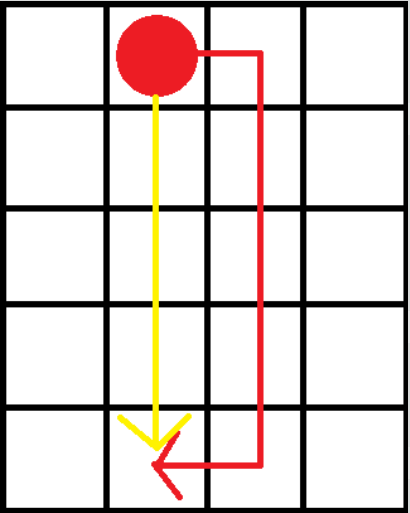
\includegraphics[scale=.4]{./General Information/canto.png}}
\caption{Pegasus Knights are mounted and have 6 movement. In other Fire Emblem games, if a Pegasus Knight takes the red path then an action, then that unit can canto up to 2 tiles, because the game calculated that only 4 tiles were actually needed to reach that tile (yellow path). Unfortunately, Three Houses will not calculate this for you, and instead, will just not let you canto, because it calculates the remaining movement as if you used up all 6 tiles. If a Wyvern Rider or Cavalier with 7 move took the same red path and an action, they would have 1 move left to canto in 3H, and 3 move left in all other fire emblem games.}
\end{figure}

\subsection*{The Door}
\addcontentsline{toc}{subsection}{The Door}
\begin{itemize}
\item In the early game, when controlling \Byleth\ in the Monastery for the first time, you have to talk to the three House Lords. Past \Edelgard\ is a door that seemingly randomly doesn't open for 9-10 seconds, which can cause a large early timeloss.
\item You can set up the game so that this doesn't happen by doing the following steps:
\begin{enumerate}
	\item Set up a save file in the Officer's Academy - Monastery for the first time, during the first quest
	\item Before every batch of attemps, load the save file, reset, and then start the run
	\item You don't necessarily need to open the save file before every attempt, but you'll probably want to load it again if you reset past Chapter 5 or so.
\end{enumerate}
\end{itemize}
\newcommand{\answerline}[5]{\multicolumn{1}{|c|}{\cellcolor{gray!75}#1} & \multicolumn{1}{c|}{#2} & \multicolumn{1}{c|}{#3} & \multicolumn{1}{c|}{#4} & \multicolumn{1}{c|}{#5} \\ \hline}

\section*{Lecture Questions}
\addcontentsline{toc}{section}{Lecture Questions}

Whenever possible, you want to choose the worst lecture possible, to gain the least amount of Professor Points. However, this is a minor timesave, so if you aren't sure then you're better off mashing. Each house has an position that is the on average worse, in Part 1, that if you aren't sure you should select. If you want to select the bottom option, you can buffer the ``down'' input to quickly move the cursor to there.
\begin{table}[h]
\centering
\begin{tabular}{c|c|c|c|c|}
\multicolumn{5}{c}{Black Eagles (Default: Bottom)}                                                                                                   \\ \cline{2-5} 
\multicolumn{1}{c|}{} & \multicolumn{2}{c|}{Part 1}                         & \multicolumn{2}{c|}{Part 2}                         \\ \hline
\multicolumn{1}{|c|}{Unit} & \multicolumn{1}{c|}{Best} & \multicolumn{1}{c|}{Worst} & \multicolumn{1}{c|}{Best} & \multicolumn{1}{c|}{Worst} \\ \hline
\answerline{\Edelgard}{Middle}{Bottom}{Top}{Bottom}
\answerline{\Hubert}{Middle}{Bottom}{Middle}{Bottom}
\answerline{\Dorothea}{Bottom}{Middle}{Top}{Middle}
\answerline{\Ferdinand}{Bottom}{Top}{Top}{Bottom}
\answerline{\Bernadetta}{Top}{Middle}{Top}{Bottom}
\answerline{\Caspar}{Bottom}{Top}{Top}{Middle}
\answerline{\Petra}{Middle}{Bottom}{Middle}{Top}
\answerline{\Linhardt}{Top}{Bottom}{Bottom}{Middle}
\multicolumn{5}{c}{Blue Lions (Default: Middle)}                                                                                                   \\ \cline{2-5} 
\multicolumn{1}{c|}{} & \multicolumn{2}{c|}{Part 1}                         & \multicolumn{2}{c|}{Part 2}                         \\ \hline
\multicolumn{1}{|c|}{Unit} & \multicolumn{1}{c|}{Best} & \multicolumn{1}{c|}{Worst} & \multicolumn{1}{c|}{Best} & \multicolumn{1}{c|}{Worst} \\ \hline
\answerline{\Dimitri}{Bottom}{Middle}{Bottom}{Top}
\answerline{\Dedue}{Bottom}{Middle}{Top}{Bottom}
\answerline{\Felix}{Top}{Middle}{?}{?}
\answerline{\Mercedes}{Top}{Bottom}{Middle}{Bottom}
\answerline{\Ashe}{Middle}{Top}{Bottom}{Top}
\answerline{\Annette}{Top}{Middle}{Bottom}{Top}
\answerline{\Sylvain}{Top}{Bottom}{Middle}{Bottom}
\answerline{\Ingrid}{Top}{Middle}{Middle}{Bottom}
\multicolumn{5}{c}{Golden Deer (Default: Top)}                                                                                                   \\ \cline{2-5} 
\multicolumn{1}{c|}{} & \multicolumn{2}{c|}{Part 1}                         & \multicolumn{2}{c|}{Part 2}                         \\ \hline
\multicolumn{1}{|c|}{Unit} & \multicolumn{1}{c|}{Best} & \multicolumn{1}{c|}{Worst} & \multicolumn{1}{c|}{Best} & \multicolumn{1}{c|}{Worst} \\ \hline
\answerline{\Claude}{Top}{Bottom}{Middle}{Bottom}
\answerline{\Lorenz}{Bottom}{Middle}{?}{Middle}
\answerline{\Hilda}{Middle}{Top}{Top}{Bottom}
\answerline{\Raphael}{Top}{Top}{Bottom}{Top}
\answerline{\Lysithea}{Bottom}{Top}{Top}{Bottom}
\answerline{\Ignatz}{Top}{Bottom}{Bottom}{Middle}
\answerline{\Marianne}{Bottom}{Middle}{Top}{Bottom}
\answerline{\Leonie}{Top}{Bottom}{Middle}{Bottom}
\end{tabular}
\begin{tabular}{c|c|c|c|c|}
\multicolumn{5}{c}{Church of Seiros}                                                                                                   \\ \cline{2-5} 
\multicolumn{1}{c|}{} & \multicolumn{2}{c|}{Part 1}                         & \multicolumn{2}{c|}{Part 2}                         \\ \hline
\answerline{\Manuela}{Bottom}{Middle}{Bottom}{Top}
\answerline{\Hanneman}{Middle}{Bottom}{Middle}{Bottom}
\answerline{\Seteth}{Middle}{Top}{Middle}{Bottom}
\answerline{\Flayn}{Middle}{Bottom}{?}{Top}
\answerline{\Cyril}{Top}{Bottom}{Top}{Bottom}
\answerline{\Catherine}{Middle}{Bottom}{Middle}{Top}
\answerline{\Alois}{Middle}{Bottom}{Top}{Middle}
\answerline{\Gilbert}{N/A}{N/A}{Bottom}{Top}
\answerline{\Shamir}{Top}{Middle}{Top}{Middle}
\multicolumn{5}{c}{Ashen Wolves}                                                                                                   \\ \cline{2-5} 
\multicolumn{1}{c|}{} & \multicolumn{2}{c|}{Part 1}                         & \multicolumn{2}{c|}{Part 2}                         \\ \hline
\multicolumn{1}{|c|}{Unit} & \multicolumn{1}{c|}{Best} & \multicolumn{1}{c|}{Worst} & \multicolumn{1}{c|}{Best} & \multicolumn{1}{c|}{Worst} \\ \hline
\answerline{\Yuri}{Top}{Middle}{Top}{Bottom}
\answerline{\Balthus}{Bottom}{Top}{N/A}{N/A}
\answerline{\Constance}{Top}{Bottom}{Middle}{Bottom}
\answerline{\Hapi}{Bottom}{Top}{Middle}{Top}
\answerline{\Anna}{Middle}{Bottom}{Middle}{Top}
\end{tabular}
\end{table}
\section*{RNG}
\addcontentsline{toc}{section}{RNG}

\subsection*{2RN System}
\addcontentsline{toc}{subsection}{2RN System}
\begin{itemize}
\item Three Houses uses a sequence of random numbers (RNs) between 0-99. The game pulls numbers out of this sequence to calculate combat parameters.
\item Like most FE games, the game uses a 2RN system to calculate hitrates. It takes the average of two random numbers then compares it to the displayed hitrate - in other words, hitrates you see are lies. Everything that uses hitrates uses the 2RN system, including attacks, gambits, monster AOEs, silence, and so on. Crits and crest activations do NOT use 2RN.
\item The tl;dr non-mathy version is that displayed hitrates >50\% have a higher hitrate than the game actually tells you, and displayed hitrates <50\% are actually lower than what's displayed. 
\item To see the actual hitrates for each displayed hitrate, see: https://serenesforest.net/general/true-hit/"											
\end{itemize}

\subsection*{Crest Activation and Critial Hits}
\addcontentsline{toc}{subsection}{Crest Activation and Critical Hits}
\begin{itemize}
\item Crest activations and critical hits do NOT use the 2RN system - in other words, what you get is actually what you see.
\item The RNs are rolled as such for each hit:
\begin{enumerate}
\item One RN is rolled for each crest activation - multiple crests can NOT be activated simultaneously, so I'm assuming if a crest activates, it skips the RNs for the rest of the crests.
\item Regardless of whether the crests activate or not, two RNs are rolled to calculate the hitrate via the 2RN system.
\item If and only if the attack lands, then one RN is rolled to calculate crit.
\end{enumerate}
\end{itemize}

\subsection*{Divine Pulse}
\addcontentsline{toc}{subsection}{Divine Pulse}
\begin{itemize}
\item Using \divinepulse\ not only reverts actions that occurred, but it also reverts the RNG sequence to where it originally was - in other words, if you do the same thing, you'll get the exact same result. But knowing how the RNG works will allow you to guarantee a different result, or take advantage of the RNs you do know of and apply it somewhere else. 

\item The simplest way to ensure you get a different result is to revert time with \divinepulse, attack an arbitrary enemy unit with a filler player unit, then try again - this will usually suffice and for 90\% of your cases, this should be enough. But maybe you did this already and you still aren't getting the result you want? Here's a detailed example:
\begin{itemize}
\item \Byleth\ attacks the \enemy{Death Knight} and get an unfavorable outcome where you miss and don't kill him. As a point of reference, let's call the starting RN for this exchange as ``RN \#1''.

\item You now revert time to just before attacking the \enemy{Death Knight}. You try the following options:

\item Attack a generic enemy unit with \Shamir\ - she has no crest, she attacks only once and lands her hit, and she doesn't get countered. This burns exactly 3 RNs (2 for her hit, 1 for her crit). You're now attacking the \enemy{Death Knight} starting at RN \#4, but you still don't kill him :(

\item Attack a generic enemy with \Hubert\ - he has no crest, he lands his one hit, and he doesn't get retaliated. This will give exactly the same result as the \Shamir\ example, since this still burns exactly 3 RNs.

\item Attack a generic enemy with \Felix\ - he has a crest but still only attacks once and lands his hit and doesn't get countered. This exchange rolled an extra RN thanks to his Crest of Fraldarius, so now you'll be on RN \#5, providing a different result when you attack the \enemy{Death Knight}

\item Double attack a generic enemy with \Petra\ - she has no crest, but she double attacks, lands her hits, and doesn't get countered, so this rolls a total of 6 RNs. Now you're on RN \#7, which is a different set of RNs from all of the above examples.

\item \Ingrid\ attacks someone up close - she attacks normally and lands it (3RNs) and the enemy retaliates but misses (2RNs), then she double attacks and lands it (3RNs). Now you're on RN \#9.
\end{itemize}
\item You generally have plenty of options to go with - the main point is to avoid wasting time and divine pulses with burns you already know the result of, such as the \Shamir\ and \Hubert\ examples.
\item You can NOT RN burn for different level ups (you CAN exit the game and re-enter the map to reroll levels, but that wouldn't happen in a speedrun)
\item Cursor movement does NOT affect the RNG, so if you're concerned about having to do fancy cursor shenanigans like the GBA FE speedruns, you don't have to.
\end{itemize}
\newpage
\setlist[enumerate]{label={Turn \arabic*:\newline}, align=left}
\chapter{Chapter 1 - The Fourth House}

\begin{itemize}
\item Difficulty: Normal/Casual
\item Male \Byleth
\end{itemize}

\begin{battle}{The Fourth House}
\begin{multicols}{2}

\battleinfo{commander}{9}{\Byleth, \Ashe, \Linhardt, \Dimitri, \Claude}
\prep{
	\item Options:
	\begin{itemize}
		\item Combat Animations:	Off \arrow{right}{1}
		\item Assist Animations: Off
		\item Battle Speed: Fast
		\item Action Skip: On
		\item Automatic Cursor: Off
	\end{itemize}
	\abilities{
		\Bylethf
		\removeAbility{Battalion Vantage}
		\addAbility{HP+5}
		\Dimitrif \arrow{right}{2}
		\removeAbility{Authority Level 3, Battalion Wrath}
		\addAbility{HP+5, Dexterity+4}
		\Claudef \arrow{right}{1}
		\addAbility{Authority Level 3, Battalion Desparation}
		\removeAbility{HP+5, Dexterity+4}
	}
	\armory{
		\Dimitrif
		\buy{2 Silver Lances}
		\Claudef
		\buy{1 Silver Bow}
	}
}

\begin{enumerate}
\turn{
	\Ashef \arrow{left}{2}
	\movegambit{3L, 2D}{Retribution}{\Hilda}{1R}
	\Dimitrif \arrow{\right}{3}
	\movegambit{1U, 7R}{Assault Troop}{\enemy{Rogue}}{1R}
	\turnend	
}
\turn{
	\Linhardtf \arrow{right}{1}
	\movephysic{4R}{\Dimitri}{}
	\Dimitrif \arrow{left}{1}
	\moveattack{1R}{\Balthus}{1R with Silver Lance}
	\movewait{5D, 2R}
	\autoCharge
}
\turn{
	\Linhardtf \arrow{right}{2}
	\movephysic{4R}{\Dimitri}{}
	\autoCharge
}
\columnbreak
\turn{
	\Claudef
	\movewait{5R - 1D, 1L from the Gate, which is 2D, 4L from \Hapi. Actual travelling will be different based on where Charge placed everyone.}
	\autoCharge
	\Dimitrif
	\begin{itemize}
		\item When the Door Key is picked up, send the Iron Lance into the Convoy.
	\end{itemize}
}
\turn{
	\Dimitrif \arrow{right}{2}
	\moveattack{2R, 4U}{\enemy{Rogue}}{1U, with the more worn-down Silver Lance}
	\Linhardtf \arrow{left}{2}
	\movephysic{Upper-Right Corner}{\Dimitri}{\arrow{right}{1}}
	\turnend
}
\turn{
	\Dimitrif \arrow{right}{2}
	\moveattack{1R, 5U}{\enemy{Archer}}{1L}
	\Linhardtf \arrow{right}{1}
	\begin{itemize}\physic{\Dimitri}{\arrow{left}{1}}\end{itemize}
	\turnend
}
\turn{
	\Dimitrif \arrow{left}{1}
	\movewait{4L, 1U}
	\begin{itemize}
	\item If there are any remaining enemies, kill them and then Canto to the avoid tile to the right of the left hole.
	\end{itemize}
	\Linhardtf \arrow{right}{1}
	\begin{itemize}\physic{\Dimitri}{\arrow{right}{1}}\end{itemize}
	\turnend
}
\turn{
	\Dimitrif \arrow{left}{1}
	\moveattack{1U}{\Constance}{1U with Javelin and Tempest Lance}
	\movewait{1U}
	\Linhardtf \arrow{right}{1}
	\begin{itemize}\physic{\Dimitri}{\arrow{right}{1}}\end{itemize}
	\turnend
}
\turn{
	\Dimitrif \arrow{left}{1}
	\moveattack{3U}{\Yuri}{1R with Silver Lance and Knightkneeler. If it isn't a one-shot, use Tempest Lance instead.}
	\ifc{\Dimitri\ fails to kill \Yuri}{\item \divinepulse \item Burn a RN with \Linhardt's Physic}
	\ifc{\Dimitri\ still fails to kill \Yuri}{\item \divinepulse \item Try Gambiting \Yuri\ instead from 1U above \Yuri}
}
\end{enumerate}

\end{multicols}

\end{battle}
\chapter{Chapter 2 - Ambush in the Arena}

\begin{battle}{Ambush in the Arena}
\begin{multicols}{2}

\battleinfo{rout}{10}{\Byleth, \Ashe, \Linhardt, \Dimitri, \Claude}
\prep{
	\item Replenish \Dimitri's Battalion, either through the prompt of his battalion broke in the previous chapter or through the Battalion Guild
	\item \Claude\ needs 29 strength by the end this chapter.
}

\begin{enumerate}
\turn{
	\Dimitrif 
	\moveattack{1R, 3U}{Grapper}{1U with Silver Lance and Knightkneeler. If you can one-shot with Steel Lance then do so instead.}
	\movewait{2U, 1L}
	\ifc{\Dimitri\ misses}{\item \divinepulse and do \Ashe's attack first.}
	\Ashef \arrow{right}{2}
	\moveattack{1L, 3U}{Grappler}{1L, 2U with Iron Bow and Curved Shot}
	\autoCharge
}
\turn{
	\Linhardtf \arrow{right}{1}
	\begin{itemize}
		\move{4U}
		\item Restore \Dimitri\ if he's rattled
	\end{itemize}
	\Ashef \arrow{right}{4}
	\movegambit{2U}{Retribution}{\Dimitri}{1U}
	\Balthusf \arrow{right}{2}
	\onlyattack{Assassin}{1D}
	\Dimitrif \arrow{left}{2}
	\onlyattack{Mercenary}{1L with the Silver Lance}
	\movewait{8U}
	\Bylethf \arrow{right}{2}
	\movewait{3D, 2L}
	\Claudef \arrow{left}{1}
	\onlyattack{Any Enemies that are nearby}{}
	\ifc{\Constance\ and \Hapi\ died}{%
		\move{3R of \Balthus}
		\wait
	}
	\ifc{\Constance\ and \Hapi\ didn't die}{%
		\move{1U, 3R of \Balthus}
		\wait
	}
	\turnend
}
\turn{
	\Dimitrif \arrow{right}{1}
	\begin{itemize}
		\move{4U}
		\item Discard the more Worn Down Silver Lance
		\equip{Silver Lance}
		\wait
	\end{itemize}
	\Claudef \arrow{left}{4}
	\moveattack{4U}{Assassin}{2R}
	\movewait{2U}
	\Linhardtf \arrow{right}{1}
	\movephysic{1L, 3U}{\Claude}{\arrow{left}{1}}
	\columnbreak
	\Bylethf \arrow{left}{1}
	\movewait{1D, 4L}
	\turnend
}
\turn{
	\Bylethf
	\movewait{4L}
	\Dimitrif \arrow{right}{1}
	\movewait{4L}
	\Claudef \arrow{right}{1}
	\movedismountuse{7L}{Concoction}
	\Linhardtf \arrow{right}{1}
	\movephysic{1U, 3L}{\Dimitri\ or \Claude}{}
	\turnend
}
\turn{
	\Linhardtf
	\movephysic{1U, 3L}{\Dimitri\ or \Claude}{}
	\Dimitrif \arrow{left}{1}
	\movewait{8L}
	\Claudef \arrow{right}{1}
	\moveattack{4L, 1D}{Mercenary}{2L with Silver Bow}
	\turnend	
}
\turn{
	\Claudef
	\moveattack{4D, 1L}{Valkyrie}{3L with Curved Shot}
	\ifc{the attack misses}{\item \divinepulse\ and burn an RN with \Linhardt}
	\turnend
}
\turn{
	 \Dimitrif \arrow{left}{2}
	 \moveattack{2L}{Last Mage}{1L}
	 \movewait{3D, 2L}
	 \Claudef \arrow{right}{2}
	 \moveuse{2D}{Concoction}
	 \turnend
}
\turn{
	\Dimitrif \arrow{right}{4}
	\moveattack{5D, 1L}{Mage}{1U}
	\movewait{1D}
	\Claudef \arrow{right}{4}
	\onlyattack{Archer}{1U, 1L with Steel Bow}
	\turnend
}
\turn{
	\Claudef
	\onlyattack{Mercenary}{1D, 1L}
	\turnend
}
\turn{
	\Claudef
	\moveattack{2U}{Mercenary}{1U, 1R}
}

\end{enumerate}

\end{multicols}

\end{battle}
\chapter{Chapter 3 - Search for the Chalice}

\begin{battle}{Search for the Chalice}
\begin{multicols}{2}

\battleinfo{Special}{7}{\Byleth, \Ashe, \Linhardt, \Dimitri, \Claude, \Yuri}
\prep{
	\inventory{
		\Bylethf
		\begin{itemize}
			\trade{\Yuri}{Iron Sword}{Fetters of Dromi}
		\end{itemize}
	}
	\map{
		\swap{\Claude}{\Linhardt}
		\swap{\Balthus}{\Dimitri}
	}
	\item Make sure that you Convoy the \textbf{Spellbreak Key} when it drops.
}

\begin{enumerate}
\turn{
	\Ashef
	\movegambit{3L, 1D}{Retribution}{\Byleth}{1D}
	\Dimitrif
	\movewait{2D}
	\Yurif
	\begin{itemize}
		\move{1U, 4R}
		\item Combat Arts: Foul Play \Byleth
	\end{itemize}
	\Bylethf
	\moveequip{4R}{Steel Sword}
	\turnend	
}
\turn{
	  \Bylethf
	  \moveattack{4D}{Paladin}{2D}
	  \movewait{1L}
	  \Claudef
	  \moveattack{3D, 1L}{Golem's Upper-Right Barrier}{2D with Monster Blast}
	  \movewait{2U}
	  \Linhardtf
	  \begin{itemize}
	  	\move{2R}
	  	\equip{Heal}
	  	\physic{Byleth}{\arrow{right}{2}}
	  \end{itemize}
	  \Yurif
	  \moverecover{1L, 2D}{\Dimitri}{1D}
	  \turnend
}
\columnbreak
\turn{
	\Linhardtf
	\begin{itemize}
		\physic{\Dimitri}{\arrow{left}{1}}
	\end{itemize}
	\Bylethf
	\movewait{1L, 5D}
	\turnend
}
\turn{
	 \Bylethf
	 \moveuse{1R, 4D}{Concoction}
	 \Yurif
	 \begin{itemize}
	 	\recover{\Dimitri}{1D}
	\end{itemize}
	\turnend
	\item Convoy the \textbf{Spellbreak Key} when it drops.
}
\turn{
	\Bylethf
	\moveattack{4D}{Soldier}{2D}
	\turnend
}
\turn{
	\Bylethf
	\begin{itemize}
		\move{1R, 5D}
		\item Convoy: Trade Vulneary for \textbf{Spellbreak Key}
		\use{Vulneary}
	\end{itemize}
	\turnend
}
\turn{
	\Bylethf
	\moveuse{3R}{Lever}
}

\end{enumerate}

\end{multicols}

\end{battle}
\chapter{Chapter 4 - A Harrowing Escape}

\begin{battle}{A Harrowing Escape}
\begin{multicols}{2}

\battleinfo{Escape the Dungeon}{12}{\Byleth, \Dimitri}
\prep{
	\replenish
	\armory{
		\repair{
			\Bylethf
			\begin{itemize}
			\item Sword of the Creator
			\end{itemize}
		}
		\forge{
			\Dimitrif
			\begin{itemize}
			\item Steel Lance \arrow{right}{1} Steel Lance+
			\end{itemize}
			\Claudef
			\begin{itemize}
			\item Steel Bow \arrow{right}{1} Steel Bow+
			\end{itemize}
		}
	}
	\units{
		\remove{\Yuri, \Constance, \Edelgard, \Claude, \Ashe, \Hilda, \Linhardt, \Hapi, \Balthus, keeping only \Byleth\ and \Dimitri}
	}
}

\begin{enumerate}
\turn{
	\Bylethf
	\movewait{4D}
	\Dimitrif
	\moveequip{5R, 3D}{Steel Lance+}
}
\turn{
	\Dimitrif
	\moveuse{1R, 7D}{Lever}
	\autoCharge
}
\turn{
	\Bylethf
	\onlyattack{Dark Bishiop}{1R}
	\movewait{1R, 5D}
	\autoUnite
}
\turn{
	 \Bylethf
	 \movewait{4D, 2L}
	 \autoUnite	 
}
\turn{
	 \Dimitrif
	 \moveuse{4D, 1R}{Concoction}
	 \Bylethf
	 \movewait{1D, 5L}
}
\columnbreak
\turn{
	\Bylethf
	\moveuse{1D, 1L}{Lever}
	\movewait{4R}
	\turnend
}
\turn{
	\Bylethf
	\movewait{2U, 4R}
	\Dimitrif
	\movewait{2D, 6R}
}
\turn{
	\Dimitrif
	\moveuse{3R, 1U}{Door}
	\movewait{1U}
	\Bylethf
	\movewait{6R}
}
\turn{
	 \Dimitrif
	 \moveattack{2U}{Mage}{1U}
	 \movewait{6U}
	 \Bylethf
	 \movewait{3R, 3U}
}
\turn{
	\Bylethf
	\movewait{6U}
	\Dimitrif
	\moveuse{2R, 4U}{Concoction}
}
\turn{
	 \Dimitrif
	 \movewait{6U}
	 \Bylethf
	 \movewait{1R, 5U}
}
\turn{
	\Bylethf
	\movewait{1R, 5U}
}


\end{enumerate}

\end{multicols}

\end{battle}
\newpage
\begin{battle}{The Exalt and the King}
\battleinfo{rout}{3}{\chrom, \robin, \sully, \frederick}
\prep{
	\units{
		\remove{Lisa ($\downarrow$), Vaike ($\downarrow\rightarrow$), Miriel ($\rightarrow$), Virion ($\uparrow$), Lon'qu ($\uparrow$)}
	}
}

\begin{enumerate}
\turn{
	\pair{\chrom}{\robin}
	\robinf
	\moveattack{1R, 4U}{Fighter}{1U}
	\pair{\sully ($\leftarrow\leftarrow$)}{\frederick}
	\frederickf
	\movewait{5L, 2U}
	\pair{Maribelle ($\leftarrow$)}{\ricken}
	\item Ricken: Wait
	\turnend
}
\turn{
	\robinf
	\movewait{2U, 2L}
	\rickenf
	\movewait{4D}
	\auto
}
\turn{
	\robinf
	\movewait{2U, 2L}
	\frederickf
	\movewait{4R, 3U}
	\rickenf
	\movewait{4L, 1D}
}
\turn{
	\robinf
	\movewait{5U}
	\auto
}
\end{enumerate}

\end{battle}
\begin{battle}{Foreseer}
\battleinfo{rout}{4}{\chrom, \robin, \sully, \frederick}
\prep{
	\units{
		\remove{\ricken ($\downarrow\rightarrow$), Maribelle ($\rightarrow$), Virion ($\downarrow$), Lissa ($\leftarrow$), Lon'qu ($\leftarrow$), Vaike ($\downarrow$)}
	}
	\map{
		\robinf\ Move 3D
	}
}

\begin{enumerate}
\turn{
	\pair{\chrom}{\robin}
	\robinf
	\movewait{4L, 1D}
	\pair{\sully ($\leftarrow\leftarrow$)}{\frederick}
	\auto
}
\turn{
	\robinf
	\movewait{4D, 1L}
	\frederickf
	\movewait{1D}
	\item Panne:
	\movewait{2D}
}
\turn{
	\robinf
	\movewait{5D}
	\auto
}
\autoturn
\end{enumerate}
\end{battle}
\chapter{Chapter 7 - A Beast in the Cathedral}

\begin{battle}{A Beast in the Cathedral}
\begin{multicols}{2}

\battleinfo{commander}{4}{\Byleth, \Dimitri, \Claude, \Dimitri, \Balthus, \Linhardt, \Ashe}
\prep{
	\replenish
	\map{
		\swap{\Dimitri}{\Hapi} \arrow{right}{2}
	}
}

\begin{enumerate}
\turn{
	\Bylethf
	\movegambit{6U}{Assault Troop}{Lower Left Barrier Tile}{1U}
	\Dimitrif \arrow{right}{4}
	\movegambit{7U, Dismount}{Blaze}{Lower Center Barrier Tile}{1U}
	\autoCharge
	\item Tilt the camera a bit so that you can see if a clone is spawned that would block \Hapi's movement, then tilt it back up to reduce lag.
}
\columnbreak
\turn{
	\ifc{a clone spawned}{
		\item Use \Balthus\ to kill it
	}
	\Hapif
	\movegambit{1R, 5U}{Blaze}{Upper Right Barrier Tile}{1L}
	\autoCharge	
}
\item \ 
\begin{itemize}
	\item Keep on Auto-Battle: Charging until the \enemy{Boss} is dead.
\end{itemize}
\end{enumerate}

\end{multicols}

\end{battle}
\end{document}
